\documentclass[border=1cm]{standalone}

\usepackage{tikz}
\usetikzlibrary{calc,intersections}

\begin{document}
    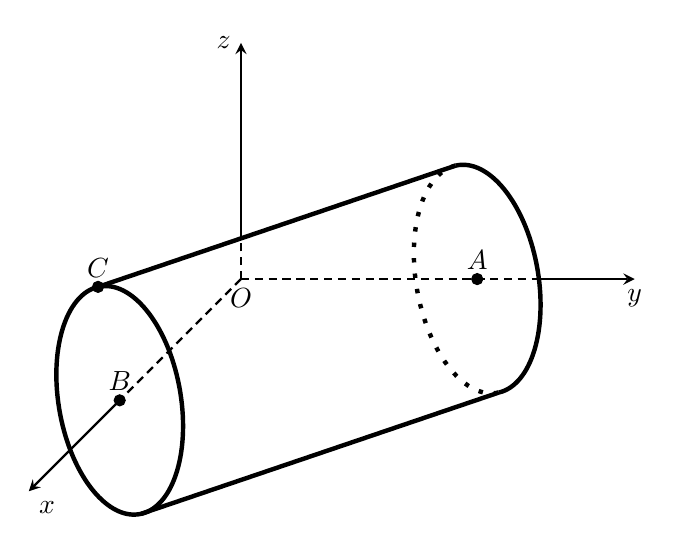
\begin{tikzpicture}
        \begin{scope}[shift={(3,0,0)},rotate around y={-90+atan(4/3)}, rotate around z=20]
            \coordinate[label=$A$] (A) at (0,0);
            \coordinate[label=$B$] (B) at (0,0,5);
            \coordinate[label=$C$] (C) at (0,{sqrt(2)},5);
            \coordinate (C1) at ($(B)+(B)-(C)$);
            \coordinate (D) at (0,{sqrt(2)},0);
            \coordinate (D1) at ($(A)+(A)-(D)$);

            \draw[ultra thick] (D1) arc [start angle=-90, end angle=90, radius={sqrt(2)}];
            \draw[ultra thick, loosely dotted] (D) arc [start angle=90, end angle=270, radius={sqrt(2)}];

            \draw[ultra thick] (B) circle [radius={sqrt(2)}];
            \draw[ultra thick] (C)--(D) (C1)--(D1);
            \draw[fill] (A) circle [radius=2pt];
            \draw[fill] (B) circle [radius=2pt];
            \draw[fill] (C) circle [radius=2pt];
        \end{scope}
        \draw[thick, densely dashed](0,0)--(3.8,0);
        \draw[->,>=stealth,thick](3.8,0)--(5,0)node[below]{$y$};

        \draw[thick, densely dashed](0,0)--(B);
        \draw[->,>=stealth,thick](B)--(0,0,7)node[below right]{$x$};

        \coordinate (Z1) at (intersection of (0,0)--(0,3) and C--D);
        \draw[thick, densely dashed] (0,0) -- (Z1);
        \draw[thick, ->, >=stealth] (Z1) -- (0,3) node[left] {\(z\)};
        \node at (0,0) [below]{$O$};

    \end{tikzpicture}
\end{document}